\documentclass{report}
\usepackage{mathptmx}
\usepackage[round]{natbib}
\usepackage{fullpage}
\usepackage{graphicx}
\usepackage[utf8]{inputenc}
\usepackage{listings}
\usepackage{mathtools, bm}
\usepackage{amssymb, bm}
\usepackage[hidelinks]{hyperref}

\renewcommand*\d{\mathop{}\!\mathrm{d}}
\renewcommand\phi{\varphi}
\renewcommand\O{\mathcal{O}}

\newcommand\bslash{\symbol{`\\}}

\DeclareMathOperator{\spn}{span}

\def\ssq{\subseteq}
\def\N{\mathbb{N}}
\def\R{\mathbb{R}}
\def\T{\mathcal{T}}
\def\iso{\text{iso}}
\def\ani{\text{ani}}
\def\mass{\text{mass}}

\begin{document}

\bibliographystyle{plainnat}
\lstset{language=Matlab}

\title{Heat and Color Flow with Finite Elements}
\author{Obed Afram, Anissa El Keurti, Robert Seidel}
\date{November 2016}
\maketitle

\tableofcontents

\listoftables

\listoffigures

\chapter{Finite Elements and the Poisson Equation}


\section{Gaussian Quadrature}

Gaussian quadrature is one of the popular integration schemes for computing integrals that are not possible to solve analytically. In one dimension the Gaussian quadrature takes the form
\begin{equation}
	\int_{-1}^{1} g(x)\d x\approx\sum_{q=1}^{Nq} \rho_q g(z_q),
\end{equation}
where $N_q$ is the number of integration points, $z_q$ are the Gaussian quadrature points and $\rho_q$ are the associated Gaussian weights. This extends to higher dimensions by
\begin{equation}
	\int_{\hat{\Omega}} g({x}) \d x\approx\sum_{q=1}^{Nq} \rho_q g(z_q),
\end{equation}
and specifying the vector quadrature points $z_q$ as well as integrating over a suitable reference domain $\hat{\Omega}$, e.g. squares or triangles in 2D, tetrahedrons or cubes in 3D.


\subsection{1D quadrature}
We write a MATLAB function \texttt{I = quadrature1D(a,b,Nq,g)}\footnote{All functions mentioned in this report can be found in the code files.} with the following arguments:
\begin{itemize}
	\item $I\in\mathbb{R}$, value of the integral,
	\item $a\in\mathbb{R}$, integration start,
	\item $b\in\mathbb{R}$, integration end,
	\item $N_q \in\mathbb{N}$, number of integration points,
	\item $g: \mathbb{R} \rightarrow \mathbb{R}$ function pointer.
\end{itemize}
We then test the written function by comparing with the analytical solution of the integral
\begin{equation}
	\int_1^2 e^x \d x = (e-1)e \approx 4.6708
\end{equation}
which happens to be the same, as the number of integration points is increased.

\subsection{2D quadrature} 

In higher dimensions, we often map to barycentric coordinates (or area coordinates, as they are known in 2D). The Gauss points are then given as triplets in this coordinate system.

We write a MATLAB function \texttt{I = quadrature2D(p1,p2,p3,Nq,g)} with the following arguments:
\begin{itemize}
	\item $I\in\mathbb{R}$, value of the integral,
	\item $p1\in\mathbb{R}^2$, first corner point of the triangle,
	\item $p2\in\mathbb{R}^2$, second corner point of the triangle,
	\item $p3\in\mathbb{R}^2$, third corner point of the triangle,
	\item $N_q \in{\{1,3,4\}}$, number of integration points,
	\item $g: \mathbb{R}^2 \rightarrow \mathbb{R}$, function pointer.
\end{itemize}
We then verify our function by comparing it with the analytical solution of the integral
\begin{equation}
	\iint \limits_{\Omega} \log (x+y) \d xdy,
\end{equation}
where $\Omega$ is the triangle defined by the corner points $(1, 0)$, $(3, 1)$ and $(3, 2)$. We solve the integral analytically by mapping the coordinates to the barycentric coordinates and compare the results.  

\begin{align}
	N_0 (\xi,\eta)&=1-\xi-\eta\\ 
	N_1 (\xi,\eta)&=\xi\\
	N_2 (\xi,\eta)&=\eta 
\end{align}

\begin{align}
	x&= P(\xi,\eta)= x_0 N_0 +x_1 N_1 +x_2 N_2 = 1+2\xi+2\eta\\
	y&= Q(\xi,\eta)= y_0 N_0 +y_1 N_1 +y_2 N_2 = \xi+2\eta\\ 
	|J| &=2
\end{align}

\begin{align}
	\iint_\Omega \log(x+y) \d xdy
	&= \iint_\Omega \log(P(\xi,\eta), Q(\xi,\eta))  \cdot |J| \d\xi \d\eta\\   
	&= \int_0^1 \int_0^{1-\eta} \log(1+3\xi+4\eta) \cdot 2 \d\xi \d\eta \approx 1.16542
\end{align}
This is approximately the same as the results from our function, with a small error when the number of integration points is increased.

\subsection{3D quadrature}

We now extend the barycentric coordinates to 3 dimensions and tetrahedral elements. We then write a MATLAB function \texttt{I=quadrature3D(p1,p2,p3,p4,Nq,g)}with the following arguments:
\begin{itemize}
	\item $I\in\mathbb{R}$, value of the integral,
	\item $p1\in\mathbb{R}^3$, first corner point of the triangle,
	\item $p2\in\mathbb{R}^3$, second corner point of the triangle,
	\item $p3\in\mathbb{R}^3$, third corner point of the triangle,
	\item $p4\in\mathbb{R}^3$, fourth corner point of the triangle,
	\item $N_q \in{\{1,4,5\}}$, number of integration points,
	\item $g: \mathbb{R}^3 \rightarrow \mathbb{R}$, function pointer.
\end{itemize}

We verify our function by comparing it with the analytical solution of the integral
\begin{equation}
	\iiint \limits_{\Omega} e^x \d x dy  \d z
\end{equation}
where $\Omega$ is the tetrahedron defined by the corner points $(0, 0, 0)$, $(0, 2, 0)$, $(0, 0, 2)$ and $(2, 0, 0)$. We solve the integral analytically by mapping the coordinates to the barycentric coordinates and compare the results with that of the numerical function which happens to be approximately the same. However, there is a little margin of error.  

\begin{align}
	N_0 (\xi,\eta,\zeta)&=1-\xi-\eta-\zeta\\ 
	N_1 (\xi,\eta,\zeta)&=\xi\\
	N_2 (\xi,\eta,\zeta)&=\eta\\
	N_3 (\xi,\eta,\zeta)&=\zeta
\end{align}

\begin{align}
	x&= P(\xi,\eta,\zeta)= x_0 N_0 +x_1 N_1 +x_2 N_2 +x_3 N_3 = 2\xi\\
	y&= Q(\xi,\eta,\zeta)= y_0 N_0 +y_1 N_1 +y_2 N_2 +y_3 N_3  = 2\eta\\ 
	z&= K(\xi,\eta,\zeta)= z_0 N_0 +z_1 N_1 +z_2 N_2 +z_3 N_3  = 2\zeta\\ 
	|J| &=6
\end{align}

\begin{align}
	\iiint_\Omega e^x \d x \d y \d z &= \iiint_\Omega e^{P(\xi,\eta,\zeta), Q(\xi,\eta,\zeta), K(\xi, \eta,\zeta)} \cdot |J| \d\xi \d\eta \d\zeta \\   
	&= \int_0^1 \int_0^{1-\xi} \int_0^{1-\xi-\eta} e^{2\xi} \cdot 6 \d\zeta \d\eta \d\xi \\
	&= \frac{3}{4}(e^2 - 5) \approx 1.79179
\end{align}


\section{Poisson in 2D}

We solve the two-dimensional Poisson problem, given by

\begin{align}
	\nabla^2 u(x,y) &= -f(x,y) \label{poissondirhom1} \\
	u(x,y)|_{\partial\Omega} &= 0 \label{poissondirhom2}
\end{align}
with $f$ given by
\begin{equation}
	f(x,y)=16\pi^2 xy(x^2 + y^2) \sin (2\pi (x^2 + y^2))-24xy\pi \cos (2\pi (x^2 + y^2)).
\end{equation}
The domain $\Omega$ is given by a three-quarter slice of the unit disc. In polar coordinates, we get
\begin{equation}
	\Omega = \{(r,\theta): r\le1 \text{ and } \theta \in [0,3\pi/2]\}.
\end{equation}

\subsection{Analytical solution}

We verify that the expression

\begin{equation} \label{poissonsol}
	u(x,y)=xy \sin (2\pi (x^2 + y^2))
\end{equation}
is a solution to the problem in (\ref{poissondirhom1}-\ref{poissondirhom2}):

\begin{align}
	\nabla^2 u(x,y) =& \frac{\partial^2 u(x,y)}{\partial x^2} + \frac{\partial^2 u(x,y)}{\partial y^2} \\
	=& \frac{\partial}{\partial x}\{y \sin (2\pi (x^2 + y^2)) +4\pi x^2 y \cos (2\pi (x^2 + y^2))\} \\
	& + \frac{\partial}{\partial y}\{x \sin (2\pi (x^2 + y^2)) +4\pi x y^2 \cos (2\pi (x^2 + y^2))\} \\
	=& 12\pi xy \cos (2\pi (x^2 + y^2)) - 16\pi^2 x^3 y\sin (2\pi (x^2 + y^2)) \\
	& + 12\pi xy \cos (2\pi (x^2 + y^2)) - 16\pi^2 x y^3 \sin (2\pi (x^2 + y^2)) \\
	=& -16\pi^2 xy (x^2 + y^2) \sin (2\pi (x^2 + y^2)) + 24\pi xy \cos (2\pi (x^2 + y^2)).
\end{align}


\subsection{Weak formulation}

We start by multiplying equation (\ref{poissondirhom1}) by a test function $v$ and integrate over the domain $\Omega$:
\begin{equation}
-\iint_{\Omega} (\nabla^2 u) v \d x \d y = \iint_{\Omega}fv \d x \d y.
\end{equation}
We apply Green's formula for the Laplacian to the first integral, with the purpose of eliminating the second derivative in order to impose a lower regularity on the solution. We find
\begin{equation}
-\iint_{\Omega} (\Delta u) v \d x \d y = \iint_{\Omega}\nabla u \cdot \nabla v \d x \d y -  \iint_{\partial \Omega} \frac{\partial u}{\partial n} v \d\gamma  
\end{equation}
We can now consider only test functions which vanish at the boundary of the domain, hence the contribution of the boundary terms vanishes. In this way, the equation becomes
\begin{equation}
\iint_{\Omega} \nabla u \cdot \nabla v \d x \d y = \iint_{\Omega}fv \d x \d y.
\end{equation}
We further reduce the equation to the form
\begin{equation}
	a(u,v) = F(v), \forall v \in V.
\end{equation}
with the bilinear functional $a$ and the linear functional $F$ given by
\begin{align}
	a(u,v) &=  \iint_{\Omega} \nabla u \cdot \nabla v \d x \d y, \\
	F(v) &= \iint_{\Omega}fv \d x \d y.
\end{align}
The space $V$ of test functions must therefore be such that if $v \in V$ then $v |_{\partial \Omega} = 0$ and $v$ must be a least once (weakly) differentiable. So, we choose $V = H_0^1(\Omega)$.

\subsection{Galerkin projection}

Instead of searching for a solution u in the entire space V, we look for a solution in a much smaller space $V_h \subset V$. We let $\Omega$ be discretized into $M$ triangles such that our computational
domain is the union of all of these, i.e. $\Omega = \bigcup_{k=1}^M$. Each triangle $K_k$ is then defined by its three corner nodes $x_i$ ($i=1,2,3$) and for each of these nodes exists a corresponding basis function. The space $V_h$ is then defined by
\begin{equation}
	V_h = \{ v \in V: v|_{K_k} \in P_1 (K_k),\ k  = 1,...,M\}
\end{equation}
for which $n \in \N$ basis functions $\{\varphi_i\}_{i=1}^n $ satisfy $V_h = \spn\{\varphi_i\}_{i=1}^n$, $\varphi_j (x_i) = \delta_{ij}$. By searching for a solution $u_h \in V_h$, it is then possible to write this as a weighted sum of the basis functions, i.e. $u_h = \sum_{i=1}^n u_h^i \varphi_i$. We now find $u_h \in V_h$ such that $a(u_h , v) = F(v)$ $\forall v \in V_h$. We arrive at the equations
\begin{align}
	a\left(\sum_{i=1}^n u_h^i \varphi_i , \varphi_j\right) &= F (\varphi_i), \\
	\sum_{i=1}^n a(u_h^i \varphi_i , \varphi_j) &= F (\varphi_i), \\
	\sum_{i=1}^n a(\varphi_i , \varphi_j) u_h^i &= F (\varphi_i),
\end{align}
which is equivalent to the linear system
\begin{equation} \label{poissondirhomlinsys}
	Au = f
\end{equation}
with
\begin{align}
	A &= [A_{ij}] = [a(\varphi_i , \varphi_j)], \\
	u &= [u_h^i], \\
	f &= [f_i] = [F (\varphi_i)].
\end{align}

\subsection{Implementation}

The function \texttt{getSlice} generates the domain $\Omega$. We apply the Gaussian quadrature in the computation and realize the computational work in the function \texttt{poisson2D\_dirichlet}. We compare here three meshes of different sizes (i.e. $n= 50, 500$ and $1000$). We observe from figure \ref{vis:2dpoissondir} that we have the image to be very close to the real solution with a very little margin of error as the number of elements is increased.

\subsubsection{Stiffness matrix}

The stiffness matrix represents the system of linear equations that must be solved in order to ascertain an approximate solution to the differential equation. In order to solve for $u$, we first choose a set of basis functions and then compute the integrals defining the stiffness matrix. We discretized the domain $\Omega$ by some form of mesh generation, wherein it is divided into non-overlapping triangles or quadrilaterals, which are generally referred to as elements. Each triangle is then visited once by the algorithm.

Without the inclusion of boundary conditions, the system (\ref{poissondirhom1}-\ref{poissondirhom2}) does not have a unique solution. Thus, the matrix $A$ is singular as well.

\subsubsection{Right hand side}

In the same manner, we build the right side vector $f$, as we did with $A$.

\subsubsection{Boundary conditions}

We implement homogeneous Dirichlet boundary conditions by deleting the boundary nodes in $A$ and $f$.

\subsection{Verification}

We solve the system (\ref{poissondirhomlinsys}) and then after verification with the analytical solution (\ref{poissonsol}), we observe that the both the solutions are approximately the same.

\section{Neumann boundary conditions}

We now change the boundary conditions of our problem to
\begin{align}
	\nabla^2 u(x,y) &= -f(x,y) \label{poissonneu1} \\
	u(x,y)|_{\partial\Omega_D} &= 0 \label{poissonneu2} \\
	\frac{\partial u(x,y)}{\partial n}|_{\partial \Omega_N} &= g(x,y) \label{poissonneu3}
\end{align}
with the source term $f$ and exact solution $u$ given as above, and $g$ defined as
\begin{equation} \label{poissonneug}
	g(x,y) = 
	\begin{cases}
	-x \sin (2 \pi x^2), & \quad y=0 \text{ and } (x,y) \in \partial \Omega_N \\
	+y \sin (2 \pi y^2), & \quad x=0 \text{ and } (x,y) \in \partial \Omega_N \\
	\end{cases}
\end{equation}
The Dirichlet boundary surface is defined in polar coordinates by $\partial \Omega_D = \{(r, \theta) : r = 1, \theta \in [0, 3 \pi /2]\}$, and the Neumann boundary surface as $\partial \Omega_N = \{(r, \theta) : r \in [-1,0], \theta = 3 \pi /2\} \cup \{(r, \theta) : r \in [0,1], \theta = 0\} $.

\subsection{Boundary condition}

We now verify that (\ref{poissonneug}) is a solution to (\ref{poissonneu1}-\ref{poissonneu3}) at the boundary.

\begin{align}
	\frac{\partial u}{\partial n} &= \nabla u \cdot \vec{n} \\
	&= \left.\frac{\partial u}{\partial x}\right|_{y=0} \cdot
	\begin{bmatrix}
		0 \\
		-1
	\end{bmatrix}
	+ \left.\frac{\partial u}{\partial y}\right|_{x=0} \cdot
	\begin{bmatrix}
		1\\
		0
	\end{bmatrix}
	& \\
	& = 
	\begin{cases}
		-x \sin (2 \pi x^2), & \quad y=0 \text{ and } (x,y) \in \partial \Omega_N \\
		+y \sin (2 \pi y^2), & \quad x=0 \text{ and } (x,y) \in \partial \Omega_N \\
	\end{cases}
\end{align}

\subsection{Variational formulation}

When we introduce a test function $v\in V =\{v\in H^1 (\Omega) : v|_{\Omega_D} = 0\}$ to (\ref{poissonneu1}-\ref{poissonneu3}), integrate over $\Omega$ and then apply Green's formula, we end up with the equation
\begin{equation}
	-\iint_{\Omega} (\Delta u) v \d x \d y = \iint_{\Omega}\nabla u \cdot \nabla v \d x \d y -  \iint_{\partial \Omega} \frac{\partial u}{\partial n} v \d\gamma = \iint_{\Omega}fv \d x \d y.
\end{equation}
We now introduce both the Dirichlet and Neumann boundary conditions
\begin{equation}
	\iint_{\Omega}\nabla u \cdot \nabla v \d x \d y = \iint_{\Omega}fv \d x \d y + \iint_{\partial \Omega_D} \frac{\partial u}{\partial n} v \d\gamma + \iint_{\partial \Omega_N} \frac{\partial u}{\partial n} v \d\gamma.
\end{equation}
By imposing that the test function $v$ vanishes on $\Omega_D$, the equation becomes
\begin{equation}
	\iint_{\Omega}\nabla u \cdot \nabla v \d x \d y = \iint_{\Omega}fv \d x \d y + \iint_{\partial \Omega_N} g v \d\gamma. 
\end{equation}
The problem takes the form:
\begin{align}
	\text{Find $u \in V$ such that } a(u,v) &= F(v) \text{ for all $v \in V$, where} \\
	a(u,v) &=  \iint_{\Omega} \nabla u \cdot \nabla v \d x \d y, \\
	F(v) &= \iint_{\Omega}fv \d x \d y + \iint_{\partial \Omega_N} g v \d\gamma.
\end{align}


\subsection{Gauss quadrature}

The Neumann boundary condition is given as an integral and must be evaluated using Gaussian quadrature. We then modify our quadrature methods from the first section to solve line integrals in two dimensions, i.e. the method signature is \texttt{I = linequadrature1D(a,b,Nq,g)} where require $a\in \mathbb{R}^2$ and $b\in \mathbb{R}^2$.

\subsection{Implementation}

We change our code to solve the Neumann boundary value problem. The solution in the interior was the same as the analytical solution. Approximately, there is a very small error comparing the solution at the boundary, see figure \ref{vis:2dpoissonneu}.

\section{Poisson in 3D}

We now solve the problem (\ref{poissondirhom1}-\ref{poissondirhom2}) in three dimensions. We then generate a mesh, using the function \texttt{getBox}, which is similar to the written function in the previous section with the only difference is that spatial coordinates have one more component. The elements now require one more index to be described. The codes from the previous section are modified to deal with the tetrahedral elements in three dimensions with a new source term $f$, defined by
\begin{equation}
	f(x,y,z) = 12\pi^2\sin (2\pi x)\sin (2\pi y)\sin (2\pi z)
\end{equation}
and homogeneous Dirichlet boundary conditions $(u^D = 0)$. The problem has the exact solution
\begin{equation}
	u(x,y,z) = \sin (2\pi x)\sin (2\pi y)\sin (2\pi z).
\end{equation}

\chapter{Anisotropic Diffusion using Finite Element Method}

After applying the Finite Element Method to common and abstract cases, we chose to work on a diffusion equation which is applied in image processing. A typical problem in image processing is \emph{denoising}. One way to remove noise in a picture is to blur noisy areas while leaving edges unchanged. The linear heat equation can be used to blur an image, as the flow of heat can be interpreted as a flow of color on a plate. However, the linear heat equation does not preserve edges. In this project, we study the effects of a nonlinear PDE in image processing: the Perona-Malik anisotropic diffusion equation, that slows down the diffusion on domains where an edge has been detected. We explain our Finite Element solver for that problem and display various numerical experiments.

\section{What is a picture?}

L infty
derivative
grad u as edge indicator

We also calculate also the PSNR by taking the initial rescaled image without noise as a reference. The PSNR (peak signal to noise ratio) is a tool that allows us to measure the quality of our reconstruction. 

\section{The Perona-Malik Equation and Finite Elements}

\subsection{Diffusion Equation}

The Perona-Malik equation \citep{perona1990} is a nonlinear diffusion equation that uses an inhomogeneous diffusivity coefficient,
\begin{equation} \label{pm}
	\frac{\partial u}{\partial t} = \nabla \cdot \left( g(\|\nabla u\|) \nabla u \right),
\end{equation}
where typical choices for $g$, often denoted as \emph{transfer function}, are
\begin{equation}
	g(\|\nabla u\|) = e^{-(\|\nabla u\|/K)^2}
\end{equation}
or
\begin{equation}
	g(\|\nabla u\|) = \frac{1}{1 + \left( \frac{\|\nabla u\|}{K}\right)^2}.
\end{equation}
Apparently, image areas with a small gradient experience strong blurring while edge areas remain unchanged. The original formulation (\ref{pm}) can lead to local backwards diffusion and become an ill-posed problem. Thus, we employ the so called \emph{regularized} Perona-Malik equation as proposed by \cite{catte1992}, where the edge indicator $\|\nabla u\|$ is replaced by $\|\nabla (G_\sigma \ast u)\|$, $G_\sigma \in C^\infty(\R^2)$ a smoothing kernel. The rest of this section relies on the definitions as given in \cite{handlovicova2002}. We begin with the regularized Perona-Malik equation
\begin{equation} \label{pmreg}
    \frac{\partial u}{\partial t} = \nabla \cdot \left( g\left(\left\|\nabla (G_{\sigma} \ast u)\right\|\right) \nabla u \right).
\end{equation}

The function $u = u(t,x)$ is defined in $I \times \Omega$. We assume $I = [0, T]$ and $\Omega \ssq \R^2$ to a bounded rectangular domain. The parameter $t$ can be seen as abstract scaling parameter \citep[p. 219]{handlovicova2002}. We equip (\ref{pmreg}) with Neumann boundary conditions
\begin{align}
	\frac{\partial u}{\partial \nu} &= 0 & \text{on } I \times \partial \Omega, \\
	u(0,x) &= {u^0}(x) & \text{in } \Omega.
\end{align}

Further, we assume $g: \R^+ \rightarrow \R^+$ to be a smooth, nonincreasing function, $g(0)=1$ and $\lim_{s \rightarrow \infty} g(s) = 0$. For the smoothing kernel, we assume $G_\sigma \in C^\infty(\R^2)$, $\int_\R G_\sigma \d x = 1$, $\int_\R |G_\sigma| \d x < \infty$ and that $G_\sigma$ converges to the Dirac measure if $\sigma \to 0$. Finally, let $u^0 \in L^\infty(\Omega)$. As described in \cite{handlovicova2002}, we do not compute the convolution $G_{\sigma} \ast u$, but use isotropic diffusion, i.e. $g \equiv 1$, in order to obtain a blurred version $u_iso$ of the image. The PDE simplifies in this case to
\begin{equation} \label{pmiso}
	\frac{\partial u_\iso}{\partial t} = \Delta u_\iso.
\end{equation}

\subsection{Finite Element Method} 

We do not present the full derivation of the Finite Element procedure in this report, but refer to the lecture and the paper from \cite{handlovicova2002}. The linear isotropic solution $u_\iso$ is used to compute the diffusion coefficients $g\left(\left\|\nabla (G_{\sigma} \ast u)\right\|\right)$. We assume these coefficients as fixed in scale, i.e. we numerically compute
\begin{equation}
	\frac{\partial u_\ani}{\partial t} = \nabla \cdot (\underbrace{g(\|\nabla \underbrace{(G_{\sigma} \ast u^0)}_{=u_\iso}\|)}_\text{const.} \nabla u_\ani).
\end{equation}

We use implicit Euler in scale and obtain the weak formulations
\begin{align}
	\int_\Omega u_\iso v \d x + \sigma \int_\Omega \nabla u_\iso \nabla v \d x &= \int_\Omega u^0 v \d x, \\
	\int_\Omega u_\ani v \d x + \tau \int_\Omega g(\|\nabla u_\iso\|) \nabla u_\ani \nabla v \d x &= \int_\Omega u^0 v \d x.
\end{align}

We consider a triangulation $\T_h$ of $\Omega$ and a nodal basis of continuous, piecewise linear functions $\phi_j$, satisfying $\phi_j(x_i) = \delta_{ji}$ for all nodes $x_i$ of $\T_h$, $i,j=1,...,M$. The initial value $u^0$ and the unknown functions $u_\iso$ and $u_\ani$ are represented by
\begin{align}
	u^0_h & = \sum_{i=1}^{M} u^0_i \phi_i, \\
	u_{\iso, h} &= \sum_{i=1}^{M} u_{\iso, i} \phi_i, \\
	u_{\ani, h} &= \sum_{i=1}^{M} u_{\ani, i} \phi_i,
\end{align}
with the unknown scalar coefficients $u^0_i, u_{\iso, i}, u_{\ani, i} \in \R$, $i=1,...,M$. With the Ritz-Galerkin method, we obtain
\begin{align}
	\sum_{i=1}^{M} \left( \int_\Omega \phi_i \phi_j \d x + \sigma \int_\Omega \nabla \phi_i \nabla \phi_j \d x \right) u_{\iso, i} &= \sum_{i=1}^{M} \left( \int_\Omega \phi_i \phi_j \d x \right) u^0_i, \\
	\sum_{i=1}^{M} \left( \int_\Omega \phi_i \phi_j \d x + \tau \int_\Omega g(\|\nabla u_{\iso,h}\|) \nabla \phi_i \nabla \phi_j \d x \right) u_{\ani, i} &= \sum_{i=1}^{M} \left( \int_\Omega \phi_i \phi_j \d x \right) u^0_i.
\end{align}
This can also be written as two linear systems
\begin{align}
	[M + \sigma A(1)] \begin{bmatrix}u_{\iso,1}\\\vdots\\u_{\iso,M}\end{bmatrix} &= M \begin{bmatrix}u^0_1\\\vdots\\u^0_M\end{bmatrix}, \\
	[M + \tau A(g(\|\nabla u_{\iso,h}\|))] \begin{bmatrix}u_{\ani,1}\\\vdots\\u_{\ani,M}\end{bmatrix} &= M \begin{bmatrix}u^0_1\\\vdots\\u^0_M\end{bmatrix},
\end{align}
where $M_{j,i} = \int_\Omega \phi_i \phi_j \d x$ is the so-called \emph{mass matrix} and $A(w)_{j,i} = \int_\Omega w \nabla \phi_i \nabla \phi_j \d x$ is the \emph{stiffness matrix}. The parameters $\sigma$ and $\tau$ denote the scale parameter for the two diffusion processes.

\section{Numerical experiments}

\subsection{First steps} 

We performed several numerical simulations of the Perona-Malik diffusion using the Finite Element Method on 2D images. Our first sample is the \texttt{cameraman} picture, see Figure \ref{cameraman}. We just write $u^0 \in \R^{n_1 \times n_2}$ from now on, to denote the initial data, where $n_1, n_2 \in \N$ denote the image dimensions.

NOISE GENERATION

We use a noisy image (by adding a random noise of parameter ${\sigma}_{noise}$) and we choose the scale of the initial image. In the figure \ref{g1-1}, the first image in the left represents the initial image that has been rescaled and added noise. The second image shows the mesh grid. Finally the two last images use two different interpolation methods on the grid, that will be developed later. \\

\paragraph{Triangular Mesh}

A naive approach for grid generation is to identify each pixel in the image with a node on the grid. The obtained squares are crossed diagonally to obtain triangles. This procedure yields a grid with $\O(n_1 n_2)$ nodes and $\O(2 n_1 n_2)$ elements. It turns out handy to use the matrix indices as spatial coordinates, i.e. we set $\Omega = [1,n_1] \times [1,n_2]$ and the triangulation nodes $x_{i,j} = (i,j)$ for $i=1,...,n_1$, $j=1,...,n_2$, see figure \ref{gridptpix}.
\begin{figure}[h]
	\centering
	\begin{tabular}{|c|c|c|}
		\hline		
		$(1,1)$ & $\hdots$ & $(1,n_2)$ \\ \hline
		$\vdots$ & $\ddots$ & $\vdots$ \\ \hline
		$(n_1,1)$ & $\hdots$ & $(n_1,n_2)$ \\ \hline
	\end{tabular}
	\caption{Matching of grid points and pixels.}
	\label{gridptpix}
\end{figure}

We realized this grid generation procedure with the function \texttt{getSquareTri} that takes the dimensions of the picture \texttt{nx} as parameters and returns \texttt{p}, a list of node coordinates, \texttt{tri}, a list of all triangles, denoted by their corner node ids, and \texttt{edge}, the set of all boundary line segments, denoted by the node ids of their corresponding start and ending points.

\paragraph{Algorithm}

The first program we tested is basically a modified version of Part 1 of the project. First, we compute the grid and pass the following arguments to \texttt{pm\_tri}:
\begin{itemize}
    \item
    \texttt{u}, the initial data,
    
    \item 
    \texttt{tri, p, edge}, the output of \texttt{getSquareTri} or another grid generator (see section
     \ref{gridgen}),
     
    \item
    the scale parameters \texttt{sigma} and \texttt{tau},
    
    \item
    the transfer function \texttt{g} as a function handle.
\end{itemize}
The function returns the followings values:
\begin{itemize}
    \item 
    \texttt{u\_ani}, the anisotropic solution,
    \item
    \texttt{A\_iso}, the isotropic stiffness matrix,
    \item
    \texttt{M}, the mass matrix,
    \item
    \texttt{u\_iso}, the isotropic solution,
    \item
    \texttt{g\_ani}, the diffusivity on the elements,
    \item
    \texttt{A\_ani}, the anisotropic stiffness matrix.
\end{itemize}
The algorithm can be described in the following way:
\begin{enumerate}
	\item
	\textbf{Isotropic diffusion (ID)}
	\begin{enumerate}	
		\item 
		Initialization of $M$, $A_\iso$, $N_q$.
		\item 
		For each triangle (visited once):
		\begin{itemize}
			\item
			Get the node id to identify points and basis functions.
			\item 
			Get the coordinates of the nodes \texttt{p1,p2,p3}.
			\item 
			Compute the functions $\phi_i$ ($i=1,2,3$) that land in the triangle.
			\item 
			For $i,j=1,2,3$:
			\begin{itemize}
				\item
				Define $f_\iso = \nabla \phi_i \nabla \phi_j$, a constant function.
				\item
				Update the isotropic stiffness matrix.\\
				\texttt{A\_iso(nodeID(i),nodeID(j)) += quadrature2D(p1,p2,p3,Nq,f\_iso);}
				\item
				Compute $f_\mass = \phi_i \phi_j$, a quadratic function.
				\item
				Update the mass matrix. \\
				\texttt{M(nodeID(i),nodeID(j)) += quadrature2D(p1,p2,p3,Nq,f\_mass);}
			\end{itemize}
		\end{itemize}
		\item 
		Solve the linear system \texttt{u\_iso = (M + sigma * A\_iso) \bslash\ (M * u)}.
	\end{enumerate}
	\item
	\textbf{Compute the diffusion coefficients (DC)}
	\begin{enumerate}
		\item 
		Initialization of the gradient matrix $d$.
		\item 
		For each triangle \texttt{k} (visited once):
		\begin{itemize}
			\item
			Get the node id to identify points and basis functions.
			\item 
			Get the coordinates of the nodes \texttt{p1,p2,p3}.
			\item 
			Compute the functions $\phi_i$ ($i=1,2,3$) that land in the triangle.
			\item
			For $i = 1,2,3$:
			\begin{itemize}
				\item
				Compute the local gradient $z = u_{\iso,i} \nabla \phi_i$.
				\item
				Update \texttt{d(k) += z}.
			\end{itemize}
		\end{itemize}
		\item 
		Evaluate the transfer function: \texttt{g\_ani = g(pointwise\_norm(d))}.
	\end{enumerate}
	\item
	\textbf{Anisotropic diffusion (AD)}
	\begin{enumerate}
		\item 
		Initialization of $A_\ani$.
		\item 
		For each triangle \texttt{k} (visited once):
		\begin{itemize}
			\item
			Get the node id to identify points and basis functions.
			\item 
			Get the coordinates of the nodes \texttt{p1,p2,p3}.
			\item 
			Compute the functions $\phi_i$ ($i=1,2,3$) that land in the triangle.
			\item 
			For $i,j=1,2,3$:
			\begin{itemize}
				\item
				Define $f_\ani = g_k \nabla \phi_i \nabla \phi_j$, a constant function.
				\item
				Update the anisotropic stiffness matrix.\\
				\texttt{A\_ani(nodeID(i),nodeID(j)) += quadrature2D(p1,p2,p3,Nq,f\_ani);}
			\end{itemize}
			
		\end{itemize}
		\item 
		Solve the linear system \texttt{u\_ani = (M + tau * A\_ani) \bslash\ (M * u)}.
	\end{enumerate}
\end{enumerate}

\paragraph{Visualization} 

We display our results by the following four pictures (in direction of reading):
\begin{enumerate}
	\item 
	The first picture is the initial picture.
	\item
	The second picture visualizes the used grid.
	\item
	The third picture is a visualization of the anisotropic solution $u_\ani$ on the grid using \texttt{trisurf}. We used the \emph{interpolated shading} in MATLAB to give a smooth result.
	\item
	The fourth picture represents the anisotropic solution $u_\ani$ interpolated on a regular meshgrid. We used the function \texttt{griddata} and the method \texttt{natural} for the interpolation.
\end{enumerate}
The different approaches for the visualization of $u_\ani$ become important when we use unstructured grids, see section \ref{gridgen}.

\paragraph{Results}

Our visual impression is that the image noise is removed while the edges are preserved. Table \ref{res:firsttry} summarizes the first numerical experiment.

\begin{table}[h]
	\centering
	\begin{tabular}{|ll}
		Image data & \\
		Grid generation & \texttt{getSquareTri} \\
		Num. of nodes \\
		Num. of elements \\
		Parameters & $\sigma=0.5$, $\tau=1.5$, $g(x) = e^{-(10 x)^2}$ \\
		Runtime ID \\
		Runtime DC \\
		Runtime AD \\
		PSNR \\
		Visualization & See figure \ref{vis:firsttry}. \\
	\end{tabular}
	\caption{Results of first numerical experiment}
	\label{res:firsttry}
\end{table}

\subsection{Efficient implementation}

\paragraph{Method}

In order to make a more efficient implementation, we took the following measures:

\begin{itemize}
    \item
    Precomputation and storage of triangle areas, basis function coefficients and triangle midpoints.
    \item 
    Enforce more use of vector notation.
    \item 
    Removal of the function call of \texttt{quadrature2D} and an anonymous function call. Instead, we used the precomputed values to get the triangular integral directly.
\end{itemize}

\paragraph{Results}

The program obtained is faster, see table \ref{res:efficient}. We shall use this version of the code for the further examples.

\begin{table}[h]
	\centering
	\begin{tabular}{|ll}
		Image data & \\
		Grid generation & \texttt{getSquareTri} \\
		Num. of nodes \\
		Num. of elements \\
		Parameters & $\sigma=0.5$, $\tau=1.5$, $g(x) = e^{-(10 x)^2}$ \\
		Runtime ID \\
		Runtime DC \\
		Runtime AD \\
		PSNR \\
		Visualization & See figure \ref{vis:efficient}.\\
	\end{tabular}
	\caption{Results of efficiency-improved numerical experiment}
	\label{res:efficient}
\end{table}

\subsection{Grid generation strategies} \label{gridgen}

\subsubsection{Diagonal swapping}
\paragraph{Method}
In order to fit the edges of the image better, we decided to implement an improved grid generation strategy by swapping the diagonals of some triangles. For each square that shall be divided in two triangles by \texttt{getSquareTri}, we compare the terms $|u_\text{top left} - u_\text{bottom right}|$ and $|u_\text{top right} - u_\text{bottom left}|$. If the first term is bigger than the second term, we split the square along the line through $x_\text{top right}$ and $x_\text{bottom left}$. Otherwise, we split the square along the line through $x_\text{top left}$ and $x_\text{bottom right}$. This behavior is implemented in \texttt{getSquareTri\_swp}.

\paragraph{Results}

When we compare the results with the first grid, we notice that the new grid seems to be more adapted to the image.

\begin{table}[h]
	\centering
	\begin{tabular}{|lll}
		Image data & \\
		Grid generation & \texttt{getSquareTri} & \texttt{getSquareTri\_swp} \\
		Num. of nodes \\
		Num. of elements \\
		Parameters & \multicolumn{2}{c}{$\sigma=0.5$, $\tau=1.5$, $g(x) = e^{-(10 x)^2}$} \\
		Runtime ID \\
		Runtime DC \\
		Runtime AD \\
		PSNR \\
		Visualization & See figure \ref{vis:diagonal1}. & See figure \ref{vis:diagonal2}. \\
	\end{tabular}
	\caption{Results of diagonal swapping}
	\label{res:efficient}
\end{table}





\subsubsection{Using variance information}

\paragraph{Method}

Intuitively speaking, it is not necessary to use a high resolution grid on image areas with few variation. However, the use of a fine grid is indicated in areas with high variation such as corner and edge regions. In order to use less elements in the smooth areas, and more elements in the edge areas we decided to implement a new grid generation strategy by using the \emph{variance} (as known from statistics) as criterion for the local coarseness of the grid.

We implement a recursive procedure as follows: A rectangular image portion is considered to contain enough information for grid refinement if the variance of the image portion lies above a certain threshold. If this is the case, the center of the rectangle is added as new node to the triangulation and the four resulting rectangles are analyzed recursively. We start with the whole image as initial image portion and its corner nodes as initial nodes for the mesh. The triangulation of the so generated point set is computed by MATLAB using built-in \texttt{delaunayTriangulation} procedure.

\paragraph{Further improvements}

We then added the \emph{corner value criterion} to the procedure. It also allows to perform a split if the absolute difference of any of two corner values are above a certain threshold. Finally, we set a minimal depth and maximal depth for the number of recursive function calls in order to ensure a minimal and maximal grid fineness.

and the variance gets split into four quartes when the variance of the portion is higher than a certain value and then we apply a Delaunay triangulation to the points obtained by using the function "delaunayTriangulation". We also use a corner value criterion: if any of the square's edges or the two diagonals is higher than a certain value, we split. We use the both criteria to decide if we split or not the square.  But to use this method properly, we apply first to the image a Gaussian filter (function "imgaussfilt" in Matlab with parameter $\sigma_{GaussFilt}$) to blur the initial image (and the degree of blur depends on $\sigma_{GaussFilt}$) before applying the criteria.  \\







        
        
        
\paragraph{Results}

The result given seems satisfying regarding the few numbers of nodes and elements (see figures \ref{t4} and  \ref{T4}) that are used for the reconstruction. The picture is smooth but it is difficult to distinguish the edges. 

% Table of results 

        \begin{figure}[h!]
        \centering
        \label{T4}
        \caption{Table of results with: the "Variance" grid, $scale=0.5$, $\sigma_{noise}=0.05$,$\sigma=0.5$, $\tau=1.5$}
        \begin{tabular}{|c|c|}
          \hline
         Duration &  Precomputation: 0.13s,
         Isotropic diffusion: 0.75,
         Anistropic diffusion:0.33 s   \\
        \hline
         Number of nodes & 135 \\
         \hline
         Number of elements & 259\\
 
         \hline
         PSNR & 23.88 \\
         \hline
        \end{tabular}
        \end{figure}






\subsubsection{Using the gradient}
\underline{Method}


We decided to also try a gradient criterion to create the grid. 
We use matrix convolutions (function "conv2" in Matlab) to compute the vertical and horizontal derivatives. Then we normalize the gradient obtained in order to have a number between 0 and 1, and to use it as a probability to be a node. We create a gradient mask with the nodes selected and we apply a Delaunay triangulation (delaunayTriangulation). But to use this method properly, we apply first to the image a Gaussian filter (function "imgaussfilt" in Matlab with parameter $\sigma_{GaussFilt}$) to blur the initial image (and the degree of blur depends on $\sigma_{GaussFilt}$) before applying the gradient mask. We also apply a "transfer function" $g_{grad}$ to the norm of the gradient before selecting the nodes. 







\underline{Results}

Using the "Gradient" grid gives a deeply smooth image. It results from the fact that we use the gradient twice in our analysis (once in the Perona-Malik diffusion equation, and once for the "Gradient" grid). Again, few nodes are used (see figure \ref{T5} for details). 








% Table of results 

        \begin{figure}[h!]
        \centering
        \caption{Table of results with: the "Gradient" grid, $scale=0.5$, $\sigma_{noise}=0.05$,$\sigma=0.5$, $\tau=1.5$}
        \label{T5}
        \begin{tabular}{|c|c|}
          \hline
         Duration &  Precomputation: 0.11s,
         Isotropic diffusion: 0.63,
         Anistropic diffusion:0.28 s   \\
        \hline
         Number of nodes & 197 \\
         \hline
         Number of elements & 374\\
 
         \hline
         PSNR & 22.1 \\
         \hline
        \end{tabular}
        \end{figure}






\subsection{Parameter modification}
\subsubsection{The time $\tau$}


We wanted to see the diffusion on the picture for different values of $\tau$ (figure \ref{t6}). We compare the PNSR (figure \ref{T6}) between the different values and $\tau=1.5$ seems to be the best choice, even when we compare it with other close values ($\tau=2$,$\tau=2.5$,$\tau=3$ ...). \\ 







% Table of results 

        \begin{figure}[h!]
        \label{T6}
        \centering
         \caption{Table of results for different $\tau$ with $scale=0.5$, $\sigma_{noise}=0.05$,$\sigma=0.5$ }
        \begin{tabular}{|c|c|c|c|c|c|c|c|}
        \hline
        Method & $\tau=0$ & $\tau=1.5$ & $\tau=5$ & $\tau=5$ & $\tau=10$ & $\tau=50$ & $\tau=100$
        \\ \hline
         PSNR  & 26.4 & 27.22 & 25.39 & 24.23 & 21.43 & 20.27 \\
         \hline
        \end{tabular}
        \end{figure}






\subsubsection{The coefficient $\sigma$}

Then, we wanted to study the effects of the parameter $\sigma$ from the diffusion equation on the picture. We compare the PSNR for the different values of $\sigma$ and the best choice seems to be $\sigma=0$ (see figures \ref{t7} and \ref{T7}). When we compare this choice with other close values ($\sigma=0.1$,$\sigma=0.2$...) we obtain the same result. 


       



 \begin{figure}[h!]
        \centering
        \label{T7}
         \caption{Table of results for different $\sigma$ with $scale=0.5$, $\sigma_{noise}=0.05$,$\tau=1.5$}
        \begin{tabular}{|c|c|c|c|c|c|c|}
        \hline
        Method & $\sigma=0$ & $\sigma=1.5$ & $\sigma=5$ & $\sigma=10$ & $\sigma=50$ & $\sigma=100$ \\
        \hline
        PSNR  & 30.2 & 27.3 & 24.42 & 23.8 & 23.26 & 22.8 \\
        \hline
        \end{tabular}
        \end{figure}







\subsubsection{Transfer function}


The modification of the diffusion coefficient, or more precisely the transfer function $g$ can change the way the diffusion processes on the image. We tested several transfer functions that are non-increasing and whose the limit tends toward 0. The choice of the transfer function depends on the application (deleting the noise or keeping the details for example). According to the comparison between the PSNR, the function $g= e^{-{100 x}^2}$ seems to be the best choice (see figure \ref{t8}), the picture keeps many details but is still noisy. The function $g= e^{-{10 x}^2}$ seems to give a good result with a smooth image.  \\


%https://books.google.no/books?id=JykChzLVlogC&pg=PA4&lpg=PA4&dq=anisotropic+diffusion+%22transfer+function%22&source=bl&ots=Z3VKxCW-hy&sig=NcAAOPtQ6p_ngSGSEs5GYRoLgdA&hl=fr&sa=X&ved=0ahUKEwjQ5aj0rI_QAhWE3SwKHWGnCp8Q6AEIYTAJ#v=onepage&q=anisotropic%20diffusion%20%22transfer%20function%22&f=false
%We can also use, fonction continue par morceaux -> for medical data. Depends on what we want regarding the edges etc 







% function imDifffCoeff -> plots g coeff but only on structured grids



\subsubsection{Interpolation}

We tried to modify the visualization of our results by changing the interpolation method for the anisotropic solution ("natural","nearest","linear","cubic","v4"). However we don't see any particular differences between the different interpolation methods with the "cameraman" picture. 




\subsubsection{The parameters of the grids}

For the "Variance" and "Gradient" grid, the numbers of nodes and elements are very low regarding the quality of the image. We can modify the parameters in order to increase the numbers of nodes and elements. 
For the "Variance" grid (see figure \ref{t11}), we decrease the "minimum variance" value, so more nodes can be selected. For the "Gradient grid" (see figure \ref{t12}) we can only modify the function $g_{grad}$ that we defined earlier. 






\subsubsection{The noise}


We wanted to study the different effects of our grids when we increase the noise in the initial picture. So far, if we compare the "ratio" $\frac{PSNR}{NumberOFElement}$ (important for the algorithm's speed), the grids "Variance" and "Gradient" have the best ratio.For a very noisy picture ($\sigma_{noise}=0.2$) we compare the visualizations obtained (figure \ref{t13}). We notice that the "gradient" grid has a less good quality than the other grids, the final picture seems to be even more noisy than the initial one.  







\subsection{Quadrilateral elements}

\underline{Method}

Instead of using triangles, we thought we could use squares. We performed a Finite element algorithm using squares instead of the triangles. We used analytical computations to make the code faster by computing: 

\begin{itemize}
    \item 
    The $\phi_i$ functions and their value on the integration point 
    \item 
    The integration of the $\phi_i$ functions 
    
\end{itemize}

The visualization shows: 
\begin{enumerate}
\item 
The initial noisy image ($scale=0.5$)
\item 
The isotropic solution 
\item 
The anisotropic solution
\end{enumerate}



\underline{Results}

We notice a "checkerboard" effect (figure \ref{t14} and \ref{T14}) on the visualization of the anisotropic solution. The article \cite{shukla2013} explains that the "checkerboard" effect is a common problem of the finite element method. One way to resolve it is to use a higher order finite element but that leads to more expensive program. Other methods are proposed like "the perimeter control technique", or "the patch technique" etc. 



\section{Outlook}

Our work can be applied in several fields that involve image processing. In the medical field, image processing is often used to read information from ultrasound images for example. The goal is to distinguish the layers of different tissues (in order to find a tumor for example), this can be relatively difficult when the image is very noisy. \\

We can, in a future work, apply our algorithm on 3D images or use a higher order finite element method. \\



\chapter{Conclusion}

In this work, we showed how to implement the Perona-Malik diffusion equation using Finite element methods with a relatively fast algorithm. We also showed how to reduce the numbers of elements and nodes (so the algorithm's speed) by focusing on the important zones (edges for example) by using different methods (variance and gradient). The comparison between the different methods leads to choices depending on the application chosen (medical data, picture restoration etc) since different factors have to be taken into account (quality, speed, smoothness). 

\bibliography{literature}

\appendix

\chapter{Figures for Part 1}

\begin{figure}
	\caption{Solution of the 2D Poisson equation with homogeneous Dirichlet boundary conditions.}
	\label{vis:2dpoissondir}
\end{figure}

\begin{figure}
	\caption{Solution of the 2D Poisson equation with mixed boundary conditions.}
	\label{vis:2dpoissonneu}
\end{figure}

\chapter{Figures for Part 2}

\begin{figure}
	\caption{.}
	\label{vis:firsttry}
\end{figure}

\chapter{Legacy Figures}

 \begin{figure}[h!]
 	\label{g1}
 	\centering
 	\includegraphics[scale=0.7]{g1.jpg}
 \end{figure}
 
 
 
          \begin{figure}[h!]
          	\centering
          	\label{T2}
          	\begin{tabular}{|c|c|}
          		\hline
          		Duration &  Precomputation: 0.85s,
          		Isotropic diffusion: 5.97s,
          		Anistropic diffusion:2.7 s   \\
          		\hline
          		Number of nodes & 16384 \\
          		\hline
          		Number of elements & 32258\\
          		
          		\hline
          		PSNR & 27.36 \\
          		\hline
          	\end{tabular}
          	\caption{Table of results with the pre-computed program : scale=0.5, $\sigma_{noise}=0.05$, $\sigma=0.5$, $\tau=1.5$ }
          \end{figure}
          
          %%% t1: test with test_pm_tri (and getSquareTri) + scale 0.5
          
          \begin{figure}[h!]
          	\centering
          	\label{t1}
          	\caption{Visualization with: scale=0.5, $\sigma_{noise}=0.05$  $\sigma=0.5$, $\tau=1.5$ }
          	\includegraphics[scale=0.8]{t1.jpg}
          \end{figure}
          
          %table of results 
          \begin{figure}[h!]
          	\caption{Table of results with: scale=0.5, $\sigma_{noise}=0.05$  $\sigma=0.5$, $\tau=1.5$ }
          	\centering
          	\label{T1}
          	\begin{tabular}{|c|c|}
          		\hline
          		Duration &  Isotropic diffusion: 49.6 s
          		and Anistropic diffusion:27 s   \\
          		\hline
          		Number of nodes & 16384 \\
          		\hline
          		Number of elements & 32258\\
          		\hline
          		PSNR & 27.64\\
          		\hline
          	\end{tabular}
          \end{figure}
          
          % t2.jpg test_pm_tri_pre and getSquareTri, scale=0.5, sigma=0.05
          \begin{figure}
          	\label{t2}
          	\caption{Visualization of $u_{ani}$ with the pre-computed program : scale=0.5, $\sigma_{noise}=0.05$  $\sigma=0.5$, $\tau=1.5$ }
          	\centering
          	\includegraphics[scale=0.8]{t2.jpg}
          \end{figure}
          
 
 
 
 
 
 \begin{figure}[h!]
 	\label{g1-1}
 	\caption{Visualization of the grid with ${\sigma}_{noise}=0.05$ and $scale=0.1$}
 	\centering
 	\includegraphics[scale=0.7]{g1-1.jpg}
 \end{figure}


        %t8 test_pm_tri_preG with tau=1.5, s=0.5
        \begin{figure}
        	\label{t8}
        	\centering
        	\caption{Visualization of the diffusion for different $g$ with $scale=0.5$, $\sigma_{noise}=0.05$,$\tau=1.5$, $\sigma=0.5$ }
        	\includegraphics[scale=0.2]{t8.jpg}
        \end{figure}
        
        
        
        
        
        \begin{figure}[h!]
        	\centering
        	\label{T8}
        	\caption{Table of results for different $g$ with $scale=0.5$, $\sigma_{noise}=0.05$,$\tau=1.5$, $\sigma=0.5$ }
        	\begin{tabular}{|c|c|c|c|c|c|c|}
        		\hline
        		Method & $g= e^{-10 x}$ & $g= e^{-{0.5 x}^2}$ & $g= e^{-{10 x}^2}$ & $g= e^{-{100 x}^2}$ & $g= tanh(5 x)+1$ & $g= 1-x$  \\
        		\hline
        		PSNR  & 26.32 & 22.73 & 27.22 & 28.82 & 25.37 & 23.13 \\
        		\hline
        	\end{tabular}
        \end{figure}
        
        
        
        \begin{figure}
        	\centering
        	\label{t9}
        	\caption{Visualization of the diffusion for different interpolation methods with the "Swap triangles" grid and $scale=0.5$, $\sigma_{noise}=0.05$,$\tau=1.5$, $\sigma=0.5$ }
        	\includegraphics[scale=0.2]{t9.jpg}
        \end{figure}



% g2.jpg test_getSquareTri_swp for scale=0.1
\begin{figure}
	\label{g2}
	\centering
	\caption{Visualization of the "Swap Diagonal" grid for $scale=0.1$, and $\sigma_{noise}=0.05$}
	\includegraphics[scale=0.8]{g2.jpg}
\end{figure}


%t3 test_pm_tri_pre with getSquareTri_swp scale=0.5
\begin{figure}
	\label{t3}
	\centering
	\caption{Visualization of $u_{ani}$ with: the "Swap Diagonal" grid, $scale=0.5$, $\sigma_{noise}=0.05$,$\sigma=0.5$, $\tau=1.5$}
	\includegraphics[scale=0.8]{t3.jpg}
\end{figure}





\begin{figure}[h!]
	\centering
	\caption{Table of results with: the "Swap Diagonal" grid, $scale=0.5$, $\sigma_{noise}=0.05$,$\sigma=0.5$, $\tau=1.5$}
	\label{T3}
	\begin{tabular}{|c|c|}
		\hline
		Duration &  Precomputation: 0.78s,
		Isotropic diffusion: 5.46s,
		Anistropic diffusion:2.45 s   \\
		\hline
		Number of nodes & 16384 \\
		\hline
		Number of elements & 32258\\
		
		\hline
		PSNR & 27.19 \\
		\hline
	\end{tabular}
\end{figure}



\begin{figure}
	\centering
	\label{t11}
	\caption{Visualization of the diffusion for different "Variance grid" parameters with $scale=0.5$, $\sigma_{noise}=0.05$,$\tau=1.5$, $\sigma=0.5$ }
	\includegraphics[scale=0.2]{t11.jpg}
\end{figure}

\begin{figure}
	\centering
	\label{t12}
	\caption{Visualization of the diffusion for different "Gradient grid" parameters with $scale=0.5$, $\sigma_{noise}=0.05$,$\tau=1.5$, $\sigma=0.5$ }
	\includegraphics[scale=0.2]{t12.jpg}
\end{figure}



\begin{figure}[h!]
	\label{t13}
	\centering
	\caption{Visualization of the diffusion for different grids and $scale=1$, $\sigma_{noise}=0.2$,$\tau=1.5$, $\sigma=0.5$ }
	\includegraphics[scale=0.2]{t13.jpg}
\end{figure}

        %t9 test_pm_tri_tet_pre with tau=1.5, s=0.5
        \begin{figure}
        	\label{t14}
        	\centering
        	\caption{Visualization of the diffusion for a "squares" grids and $scale=0.5$, $\sigma_{noise}=0.05$,$\tau=1.5$, $\sigma=0.5$ }
        	\includegraphics[scale=0.2]{t14.jpg}
        \end{figure}
        
        
        
        \begin{figure}
        	\centering
        	\caption{Table of results for a "squares" grids and $scale=0.5$, $\sigma_{noise}=0.05$,$\tau=1.5$, $\sigma=0.5$ }
        	\label{T14}
        	\begin{tabular}{|c|c|}
        		\hline
        		Duration &  
        		Isotropic diffusion: 6.69s,
        		Anistropic diffusion:1.95 s   \\
        		\hline
        		Number of nodes & Number of pixels nx1*nx2 \\
        		\hline
        		Number of elements & (nx1-1)*(nx2-1)\\
        		\hline
        		PSNR & 16.12 \\
        		\hline
        	\end{tabular}
        \end{figure}

\begin{figure} \label{cameraman}
	\centering
	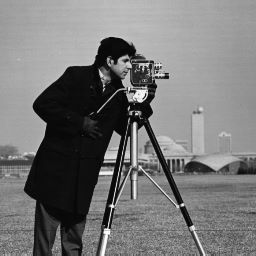
\includegraphics{cameraman.jpg}
	\caption{The \texttt{cameraman} picture}
\end{figure}

\clearpage

% g3.jpg test_getVariGrid(U,sigma=1,minvar=0.003,cvc=0.05,alldepth=3,maxdepth=50) for scale=0.1 
\begin{figure}
	\label{g3}
	\centering
	\caption{Visualization of the "Variance" grid, $scale=0.1$, $\sigma_{noise}=0.05$}
	\includegraphics[scale=0.8]{g3.jpg}
\end{figure}


% Show four pictures 

%t4 test_pm_tri_pre with getVariGrid(U,sigma=2,minvar=,cvc=,alldepth=,maxdepth=) scale=0.5 
\begin{figure}
	\label{t4}
	\centering
	\caption{Visualization of $u_{ani}$ with: the "Variance" grid, $scale=0.5$, $\sigma_{noise}=0.05$,$\sigma=0.5$, $\tau=1.5$}
	\includegraphics[scale=0.8]{t4.jpg}
\end{figure}

        % g4.jpg test_getGradGrid(U,sigma=2, g=power(x,1)) for scale=0.1 
        \begin{figure}
        	
        	\centering
        	\caption{Visualization of the "Gradient" grid, $scale=0.1$, $\sigma_{noise}=0.05$, $\sigma_{GaussFilt}=2$,  $g_{grad}=x$}
        	\includegraphics[scale=0.8]{g4.jpg}
        \end{figure}
        
        % Figure showing the final image 
        
        %t5 test_pm_tri_pre with test_getGradGrid(U,sigma=2, g=power(x,1)) for scale=0.5 
        \begin{figure}
        	
        	\centering
        	\caption{Visualization of $u_{ani}$ with: the "Gradient" grid, $scale=0.5$, $\sigma_{noise}=0.05$,$\sigma=0.5$, $\tau=1.5$}
        	\includegraphics[scale=0.8]{t5.jpg}
        \end{figure}


\clearpage

        %t6 test_pm_tri_preTau with sigma=0.5 and g idem
        \begin{figure}
        	\label{t6}
        	\centering
        	\caption{Visualization of the diffusion for different $\tau$ with $scale=0.5$, $\sigma_{noise}=0.05$,$\sigma=0.5$ }
        	\includegraphics[scale=0.2]{t6.jpg}
        \end{figure}

        %t7 test_pm_tri_preSigma with tau=1.5
        \begin{figure}
        	\label{t7}
        	\centering
        	\caption{Visualization of the diffusion for different $\sigma$ with $scale=0.5$, $\sigma_{noise}=0.05$,$\tau=1.5$ }
        	\includegraphics[scale=0.2]{t7.jpg}
        \end{figure}


\end{document}
